\documentclass[round]{bioinfo}

\usepackage{color}
\newcommand{\cred}{\color{red}}

\usepackage{url}
% \usepackage[colorlinks,citecolor=blue,linkcolor=red,urlcolor=blue]{hyperref}
\newcommand{\thefirstpage}{1} \newcommand{\thelastpage}{1}

\copyrightyear{2010}
\pubyear{2010}

\begin{document}

\firstpage{1}
\application{}
\title[ExpressionView]{ExpressionView - an interactive viewer for
  biclusters identified in gene expression data} 
\author[Andreas L\"uscher, G\'abor Cs\'ardi, Aitana Morton de
Lachapelle, Zolt\'an Kutalik, and Sven Bergmann]{Andreas
  L\"uscher$^1$, G\'abor Cs\'ardi$^{1,2}$, Aitana Morton de
  Lachapelle$^{1,2}$, Zolt\'an Kutalik$^{1,2}$, Bastian Peter$^{1,2}$
  and Sven Bergmann$^{1,2}$\footnote{to whom correspondence should be
    addressed}} 
\address{
  $^{1}$Swiss Institute of Bioinformatics, Lausanne, Switzerland\\
  $^{2}$Department of Medical Genetics, University of Lausanne,
  Lausanne, Switzerland 
}

\history{Received on XXXXX; revised on XXXXX; accepted on XXXXX}

\editor{Associate Editor: XXXXXXX}

\maketitle

\begin{abstract}

\section{Summary:}
ExpressionView is an R package that provides an interactive graphical
environment to explore biclusters identified in gene expression
data. A sophisticated ordering algorithm is used to present the
biclusters in a visually appealing layout that provides an intuitive
summary of the results. From this overview, the user can select
individual biclusters and access all the biologically relevant data
associated with it. The package is aimed to facilitate the
collaboration between bioinformaticians and life scientists.

\section{Availability:} 
%\href{http://www.unil.ch/cbg/ExpressionView}{R 
%  package with open source license,
\url{http://www.unil.ch/cbg/ExpressionView}
%} 

\section{Contact:} \href{Sven.Bergmann@unil.ch}{Sven.Bergmann@unil.ch}

\section{Supplementary information:}
Screenshots, tutorials and sample data sets can be found on the
ExpressionView \href{http://www.unil.ch/cbg/ExpressionView}{website}. 

\end{abstract}

\section{Introduction}
Biclustering is an unsupervised learning technique used to analyse
microarray data. It consists of identifying co-regulated groups of
genes and conditions according to their expression profile. While
there is a multitude of biclustering software available~(see in
\cite{madeira04}), packages with intuitive interfaces that allow the
user to interactively explore the results are
sparse~\citep{santamaria08}. ExpressionView is designed to close this
gap, and facilitate the collaboration between bioinformaticians and
life scientists without consolidated programming
experience. Implemented as an R package, the user can apply all the
powerful microarray analysis tools provided by the
Bioconductor~\citep{gentleman04} project before exporting the data to
a platform independent Adobe Flash applet that allows one to visualise
the biclusters together with the underlying gene expression data. 

\section{Package design and workflow}
The ExpressionView package contains two independent parts: An ordering
algorithm implemented in C++ and an Adobe Flash applet written in
ActionScript and Adobe Flex. Fig.~\ref{fig:workflow} schematically
summarises the typical workflow that uses the gene expression data
available as a Bioconductor ExpressionSet and combines it with the
biclustering results to produce an ExpressionView data file that can
be explored with the Flash applet. In the following, we describe the
different steps in more detail. 
\begin{figure*}[!tpb]
\centerline{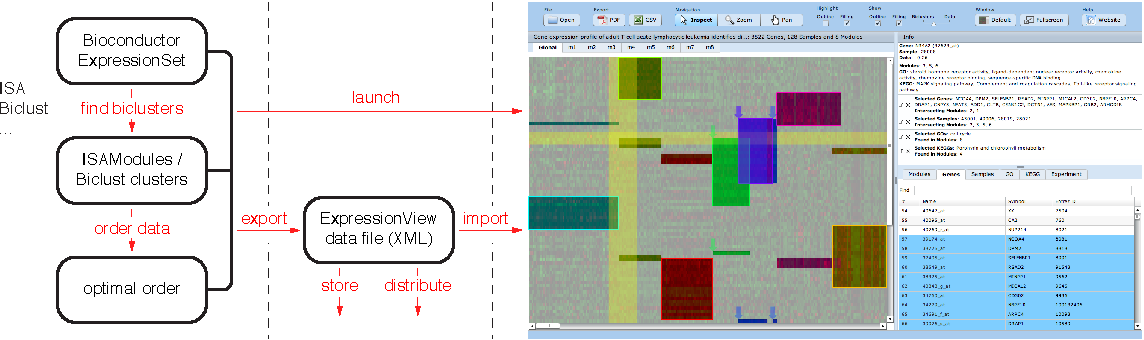
\includegraphics[width=0.9\linewidth]{fig1-crop}}
\caption{How to use ExpressionView: Starting from gene expression data
  in the form of a Bioconductor ExpressionSet, the user first runs a
  biclustering algorithm to determine co-regulated groups of genes and
  samples. In a second step, the rows and columns of the gene
  expression matrix are rearranged to produce an easily readable
  overview of the results. The last step consists of combining the
  gene expression data and its associated metadata with the results
  from the biclustering and produce an ExpressionView data file that
  can be explored with the interactive Flash
  applet.}\label{fig:workflow} 
\end{figure*}
For users who prefer to install the viewer as a standalone program, we
also provide a platform independent Adobe AIR version that can be
downloaded from the
\href{http://www.unil.ch/cbg/ExpressionView}{website}. 

\subsection{Gene expression data and biclusters}
ExpressionView is designed to work with gene expression data in the
form of a Bioconductor ExpressionSet. This class provides a
user-friendly way to access the actual gene expression matrix and its
associated metadata. There is a variety of biclustering algorithms
described in the literature~\citep{madeira04,prelic06}, several of
which have been implemented as R packages. ExpressionView can treat
results obtained by the iterative signature algorithm
(ISA)~\citep{bergmann03} %,csardi09 
and the methods available in the Biclust
package~\citep{kaiser08}. Since the structure of biclustering results
is independent of the algorithm, an extension to other methods is
straightforward. 

\subsection{Order}
To present the dozens of possibly overlapping biclusters in a visually
appealing form, it is necessary to reorder the rows and columns of the
gene expression matrix in such a way that biclusters form contiguous
rectangles. Since it is in general impossible to find such an
arrangement for more than two mutually overlapping biclusters, one has
to make concessions. In contrast to \cite{grothaus06}, who proposed to
repeat rows and columns as necessary, we prefer
to optimise the arrangement within the original data by maximising the
total area of the largest contiguous biclusters.  

Since this reordering is an interesting problem on its own, which to
the best of our knowledge has not been studied in the literature, we
briefly outline our strategy here. Noting that the rows and the
columns can be ordered independently, the problem reduces to finding
the optimal arrangement of a set of $n$ elements that are part of at
least one of $m$ clusters. The quality of the order is defined as the
sum of the maximal number of neighbouring elements in every cluster
and the aim is to maximize this quantity by changing the order of the
elements. Starting from an initial configuration determined by
hierarchical clustering, this is achieved by either shifting well
aligned subsequences of a given cluster, hence enlarging the longest
contiguous part, or permuting the individual elements of a given
contiguous block. 

To determine the efficiency of this method, we have studied a large
number of perfectly orderable, but initially scrambled, test cases. We
find that in almost every situation, the proposed algorithm finds an
order that recovers more than 99\% of the score of the optimal
solution and in most cases, it recovers the correct
alignment. For random samples, which are more representative for
actual gene expression data than orderable situations, execution time
increases polynomially with the number of clusters $m$ as ${\mathcal
  O}(m^\alpha)$, where $\alpha \in [1.6, 2]$, almost independently of
the number of elements $n$. For a given number of clusters, we find
${\mathcal O}(n^\alpha)$, with $\alpha \in [2.5, 2.7]$. 

\subsection{Export}
Once the optimal order is determined, the program rearranges the gene
expression matrix accordingly and exports all the relevant information
into an XML file. This format has the advantage of being
self-explanatory and extensible. In addition, the files can be read
and edited with any text editor. The actual gene expression data is
rounded to two digit precision and encoded in Base64. The structure of
the XML file is described in more detail on the ExpressionView
\href{http://www.unil.ch/cbg/ExpressionView}{website}. In most cases,
these files are of the order of a few Megabytes and can thus easily be
sent to co-workers.  

\subsection{Visualisation}
The core application of this package is the Flash applet that allows
the user to interactively explore the gene expression data and the
biclusters. The Flash architecture has the advantage of producing a
platform and browser independent applet that can be launched from any
computer with even the most restrictive user rights. A screenshot is
shown in Fig.~\ref{fig:workflow}. The interface is divided in two
parts: On the left-hand side, the user finds the gene expression data
in the common heat map form, on top of which the biclusters are
overlaid. On the right-hand side, the metadata associated with the
gene expression data and the results of the enrichment calculations
(Gene Ontology~\citep{ashburner00} and Kyoto Encyclopedia
of Genes and Genomes ~\citep{kanehisa04}] are shown. Wherever
possible, these elements are linked to the corresponding
databases. The interface essentially behaves as an image viewer,
allowing the user to zoom and pan around the expression data, getting
instant feedback on the selected item. The currently selected region
can be exported to a PDF file, or a simple text file.

\section*{Acknowledgement}

\paragraph{Funding\textcolon} The authors are grateful to the Swiss
Institute of Bioinformatics, the Swiss National Science Foundation
(3100AO-116323/1) and the European Framework Project 6 (through
the EuroDia and AnEuploidy projects).

\paragraph{Conflict of interest\textcolon} none declared.

\begin{thebibliography}{6}

\bibitem[Ashburner et~al.(2000)]{ashburner00}
Ashburner,M. \emph{et al.} (2000)
Gene Ontology: tool for the unification of biology.
\href{http://dx.doi.org/10.1038/75556}{\emph{Nature Genetics}, {\bf 25}, 25--29.}

\bibitem[Bergmann et~al.(2003)]{bergmann03}
Bergmann,S., Ihmels,J. and Barkai,N. (2003)
Iterative signature algorithm for the analysis of large-scale gene expression data.
\href{http://dx.doi.org/10.1103/PhysRevE.67.031902 }{\emph{Physical Review E}, {\bf 67}, 031902.}

%\bibitem[Cs{\'a}rdi et~al.(2009)]{csardi09}
%Cs{\'a}rdi,G., Kutalik,Z. and Bergmann,S. (2009)
%Modular analysis of gene expression data with R.
%\href{http://dx.doi.org/}{\emph{Bioinformatics}, ...}

\bibitem[Gentleman et~al.(2004)]{gentleman04}
Gentleman,R.C., \emph{et al.} (2004)
Bioconductor: open software development for computational biology and bioinformatics.
\href{http://dx.doi.org/10.1186/gb-2004-5-10-r80}{\emph{Genome Biology}, {\bf 5}, R80.}

\bibitem[Grothaus et~al.(2006)]{grothaus06}
Grothaus,G., Mufti,A., and Murali,TM. (2006)
Automatic layout and visualization of biclusters.
\href{http://dx.doi.org/10.1186/1748-7188-1-15}{\emph{Algorithms for Molecular Biology}, {\bf 1}, 15.}

\bibitem[Kaiser and Leisch(2008)]{kaiser08}
Kaiser,S. and Leisch,F. (2008)
A toolbox for bicluster analysis in R.
\href{http://epub.ub.uni-muenchen.de/3293/}{Technical Report 028, Department of Statistics, University of Munich}.

\bibitem[Kanehisa et~al.(2004)]{kanehisa04}
Kanehisa,M. \emph{et al.} (2004)
The KEGG resource for deciphering the genome.
\href{http://dx.doi.org/10.1093/nar/gkh063}{\emph{Nucleic Acids Res.}, {\bf 32} (Database special issue), D277.}

\bibitem[Madeira and Oliveira(2004)]{madeira04}
Madeira,S.C. and Oliveira,A.L. (2004)
Biclustering algorithms for biological data analysis: A survey.
\href{http://dx.doi.org/10.1109/TCBB.2004.2}{\emph{IEEE/ACM Transactions on Computational Biology and Bioinformatics}, {\bf 1}, 24--45.}

\bibitem[Prelic et~al.(2006)]{prelic06}
Prelic,A., \emph{et~al.} 
A systematic comparison and evaluation of biclustering methods for gene expression data 
\href{http://dx.doi.org/10.1093/bioinformatics/bt1060}{\emph{Bioinformatics}, {\bf 22}(9), 1122--1129.}

\bibitem[Santamar\'ia et~al.(2008)]{santamaria08}
Santamar\'ia,R., Ther\'on,R. and Quintales,L. (2008)
BicOverlapper: A tool for bicluster visualization. 
\href{http://dx.doi.org/10.1093/bioinformatics/btn076}{\emph{Bioinformatics}, {\bf 24}, 1212--1213.}

\end{thebibliography}

\end{document}
